\chapter{Simulation tests} %Preliminary Results
\section{Bunch parameters}
The intimal phase of this project involves simulating beam dumping of the proposed electron beam of the EuPRAXIA project. This is a European Union Horizon 2020 research project with the aim of developing a conceptual design report for a high-quality compact 5 GeV electron plasma wakefield accelerator for application in research and medicine \cite{Eupraxia}. Currently the studies are concerned with achieving high-quality 1 GeV electron beams. As the simulations and experiments yield successful results at this energy, higher energies will be expolored until the 5 GeV goal is reached. Current target values for the electron bunch parameters are given in table \ref{eupraxia_parameters}, where case 1 and 2 represents laser-driven and beam-driven driven accelerators respectively \cite{Eupraxia}.  In addition, parameters are shown for the simulated 1 GeV electron beam that we aim to dump. These differ in two key aspects to the other EuPRAXIA cases. Firstly, the energy spread and emittance of the bunch have been lowered. This lowers the computational cost of running these simulations, by effectively decreasing the relative motion of the particles in the bunch, while still maintaining a realistic beam quality \cite{Walker2017}. Secondly, the size of the bi-Gaussian bunch has been increased significantly because of the fact that the current parameters would lead to bunch densities in excess of $10^{20} \text{cm}^{-3}$, making neither linear nor quasilinear regimes accessible with conventional plasma sources. Plasma densities up to $\sim 10^{20} \text{cm}^{-3}$ are achievable using supersonic gas jets \cite{Schmid2012} -- where a a high-density gas jet is ionised into a plasma using a laser -- however the novelty and impracticality of this technique lead us to instead lowering the bunch density. Expansion of the bunch in the radial direction could be achieved by simply letting the bunch propagate freely in a vacuum, at which point the bunch would expand due to its space-charge force, while longitudinal stretching is achievable using conventional so-called magnetic chicanes \cite{Maier2012}. We choose here to expand the dimensions of the bunch to $\sigma_{\xi}=\sigma_r=5~\mu\text{m}$. This is chosen in part to give a more workable bunch density of $10^{17} \text{cm}^{-3}$, as well as to allow for comparisons with existing free-electron laser and plasma wakefield experiments, which tend to have bunch dimensions in the single to tens of micrometer range. 


\begin{table}
\centering
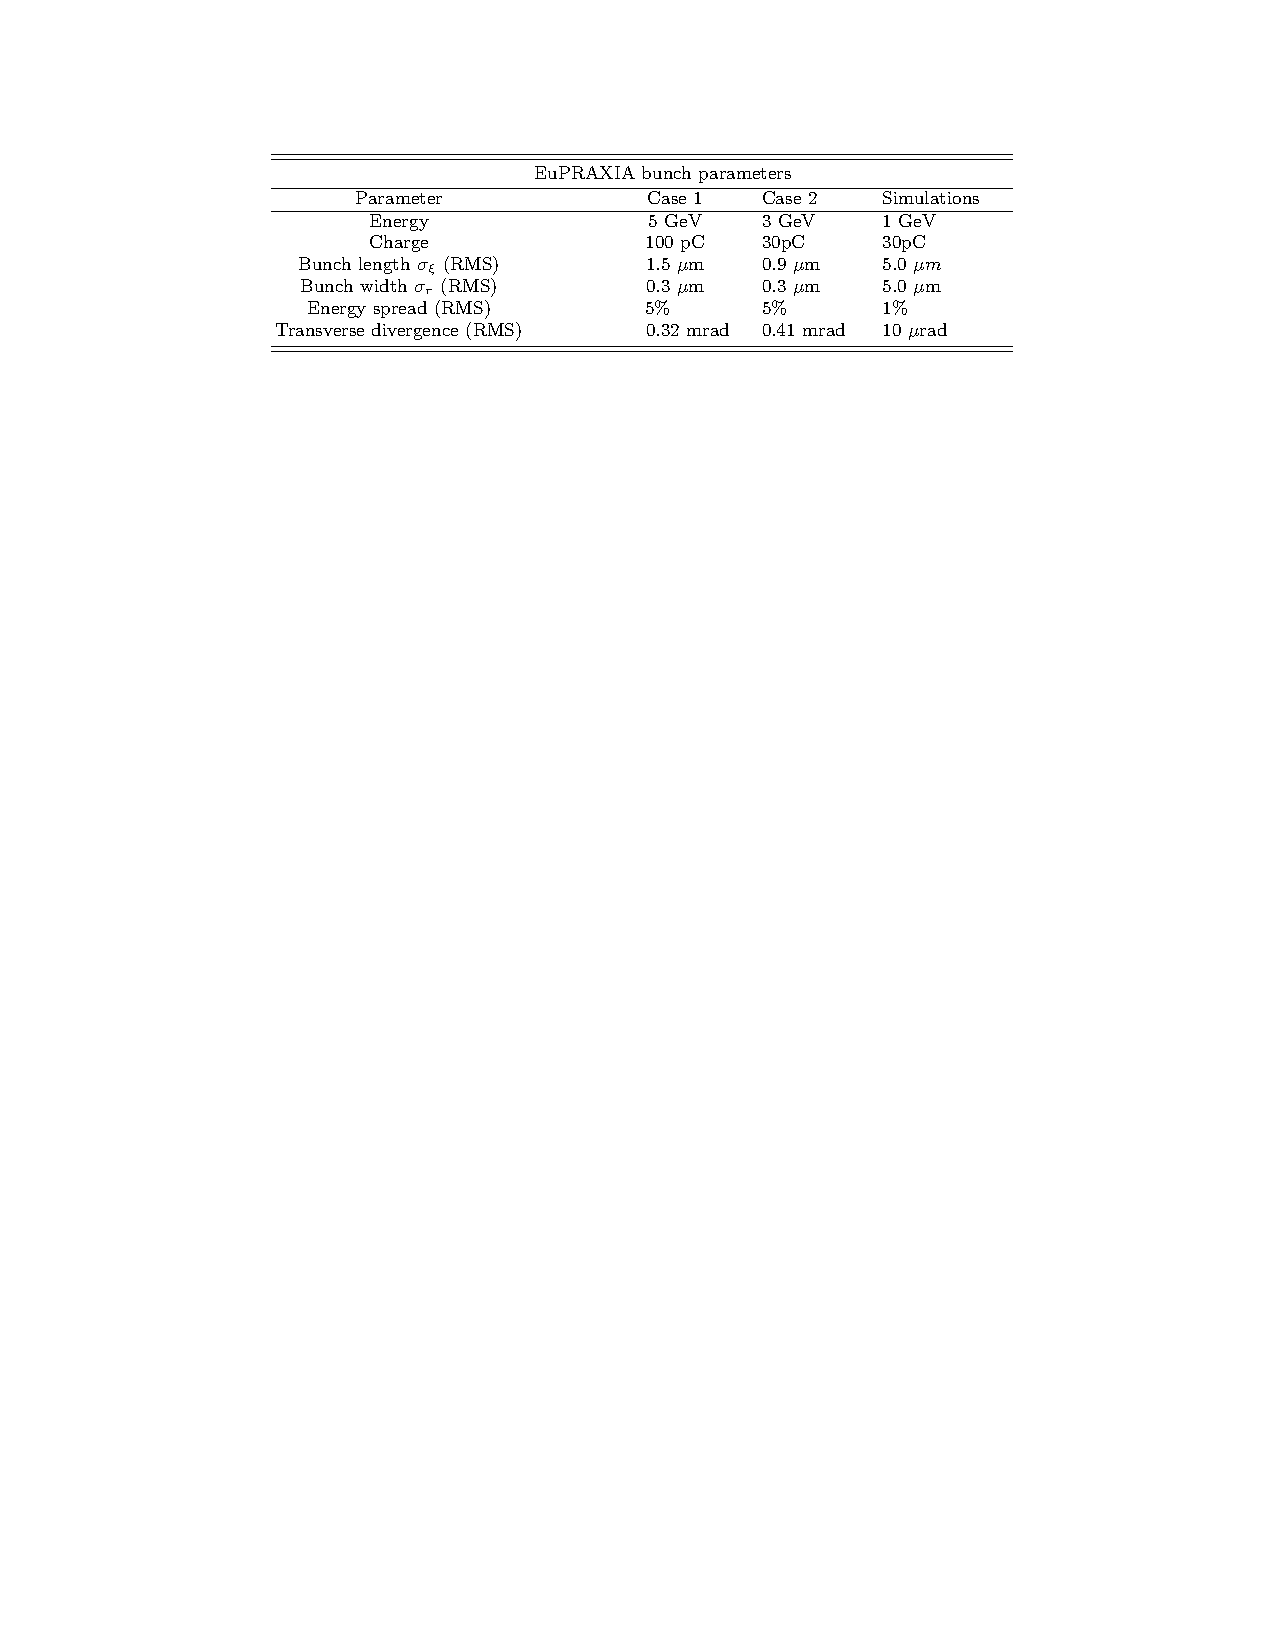
\includegraphics[width=0.85\textwidth]{table_eupraxia.pdf}
\caption{Parameters for the accelerated electron bunch in the EuPRAXIA project for laser-driven  (case 1) and beam-driven (case 2) plasma wakefield acceleration. As well as, parameters for the simulated beam used in our hybrid scheme study.}
\label{eupraxia_parameters}
\end{table}

\section{Linear and quasilinear regimes}

\begin{figure}
\centering
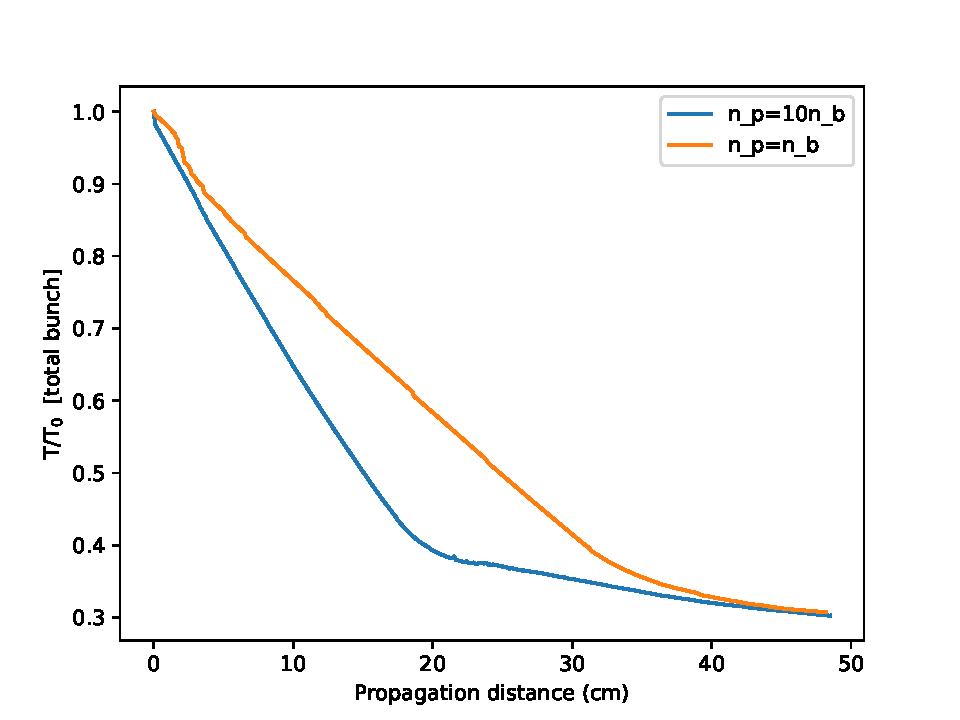
\includegraphics[width=0.49\textwidth]{Energies30pc_lowres.pdf}
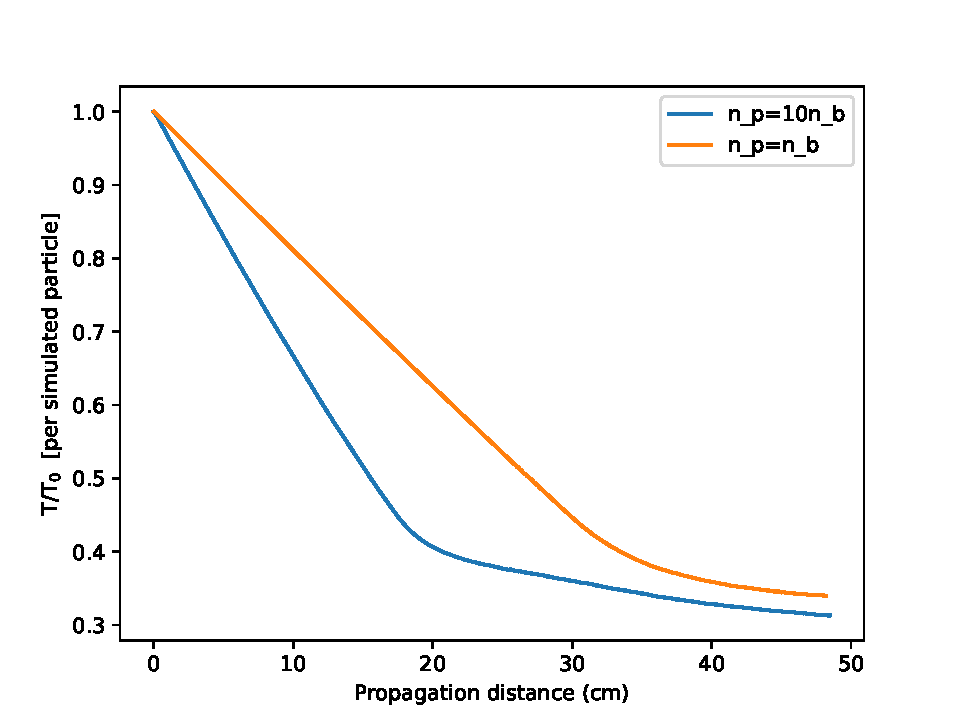
\includegraphics[width=0.49\textwidth]{Energy30pc_per_particle_lowres.pdf}
\caption{•}
\end{figure}

\begin{figure}
\centering
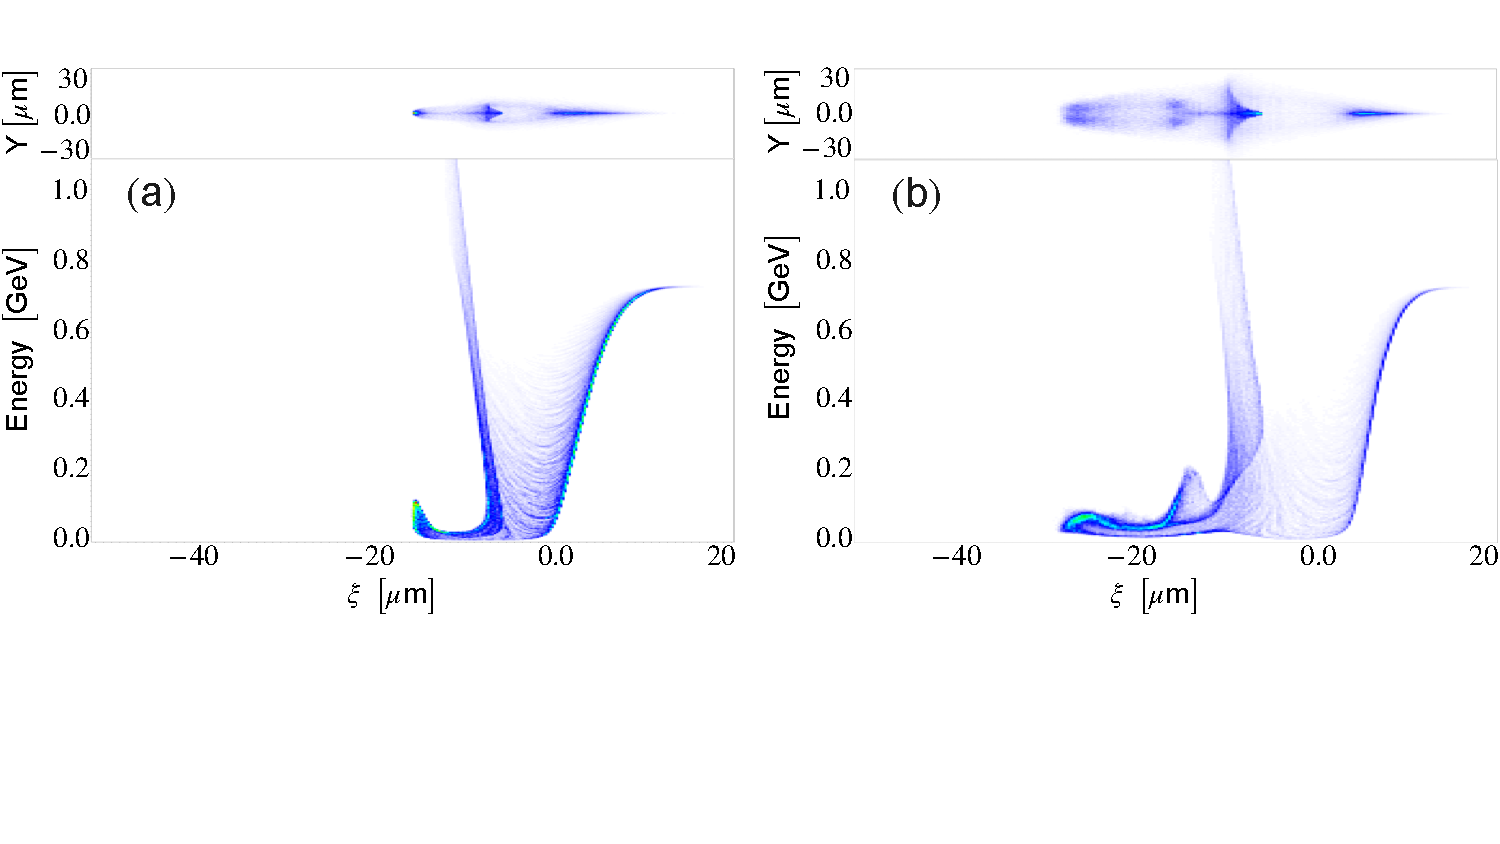
\includegraphics[width=\textwidth]{linearplots.pdf}
\end{figure}
\begin{figure}
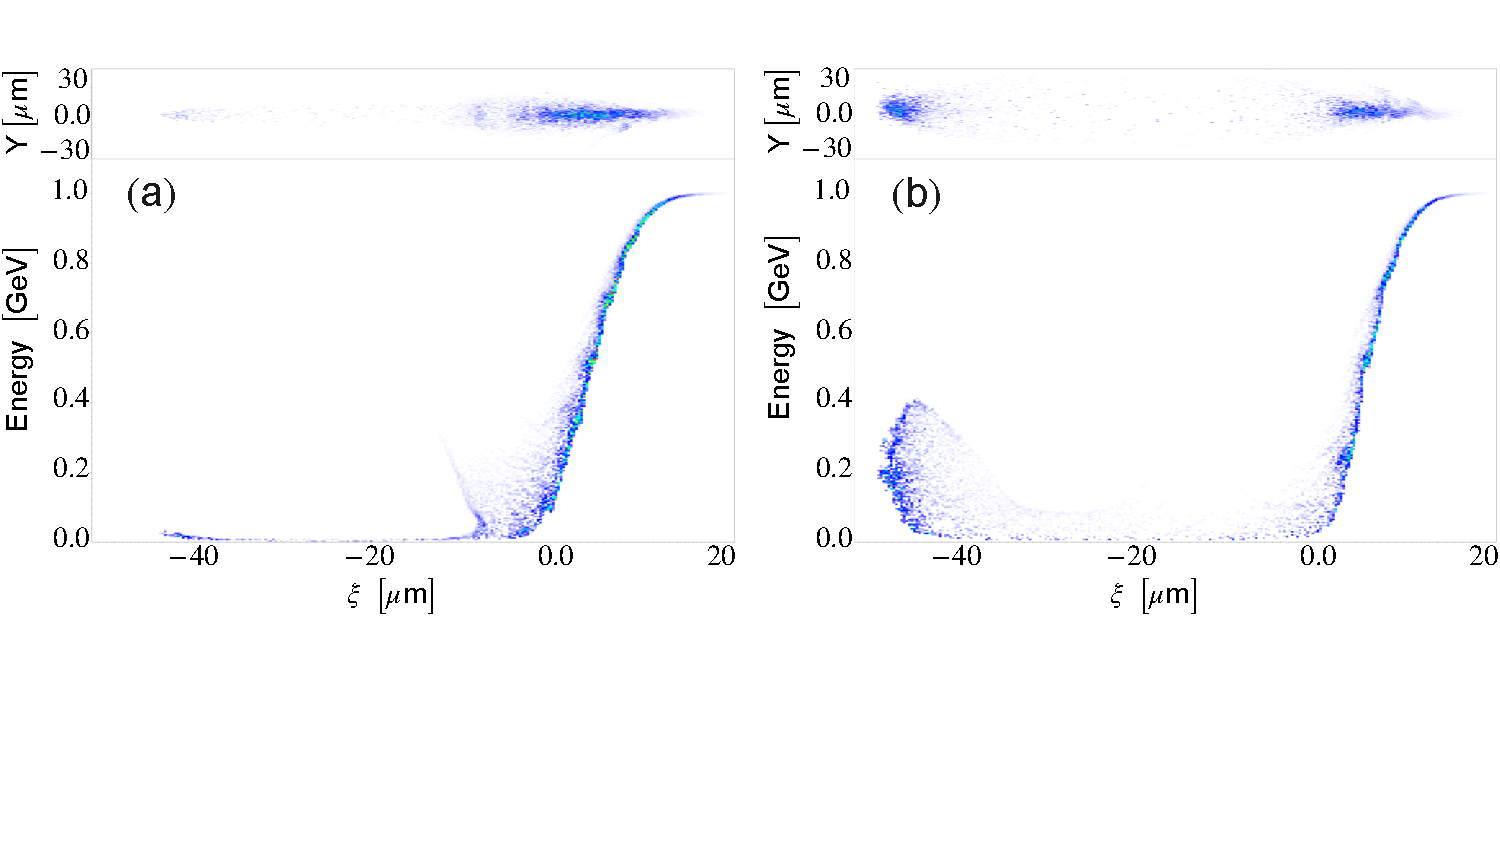
\includegraphics[width=\textwidth]{quasiplots}
\caption{quasiplots}
\end{figure}

\subsection{Transverse instabilities in quasilinear regime}
\begin{figure}
\centering
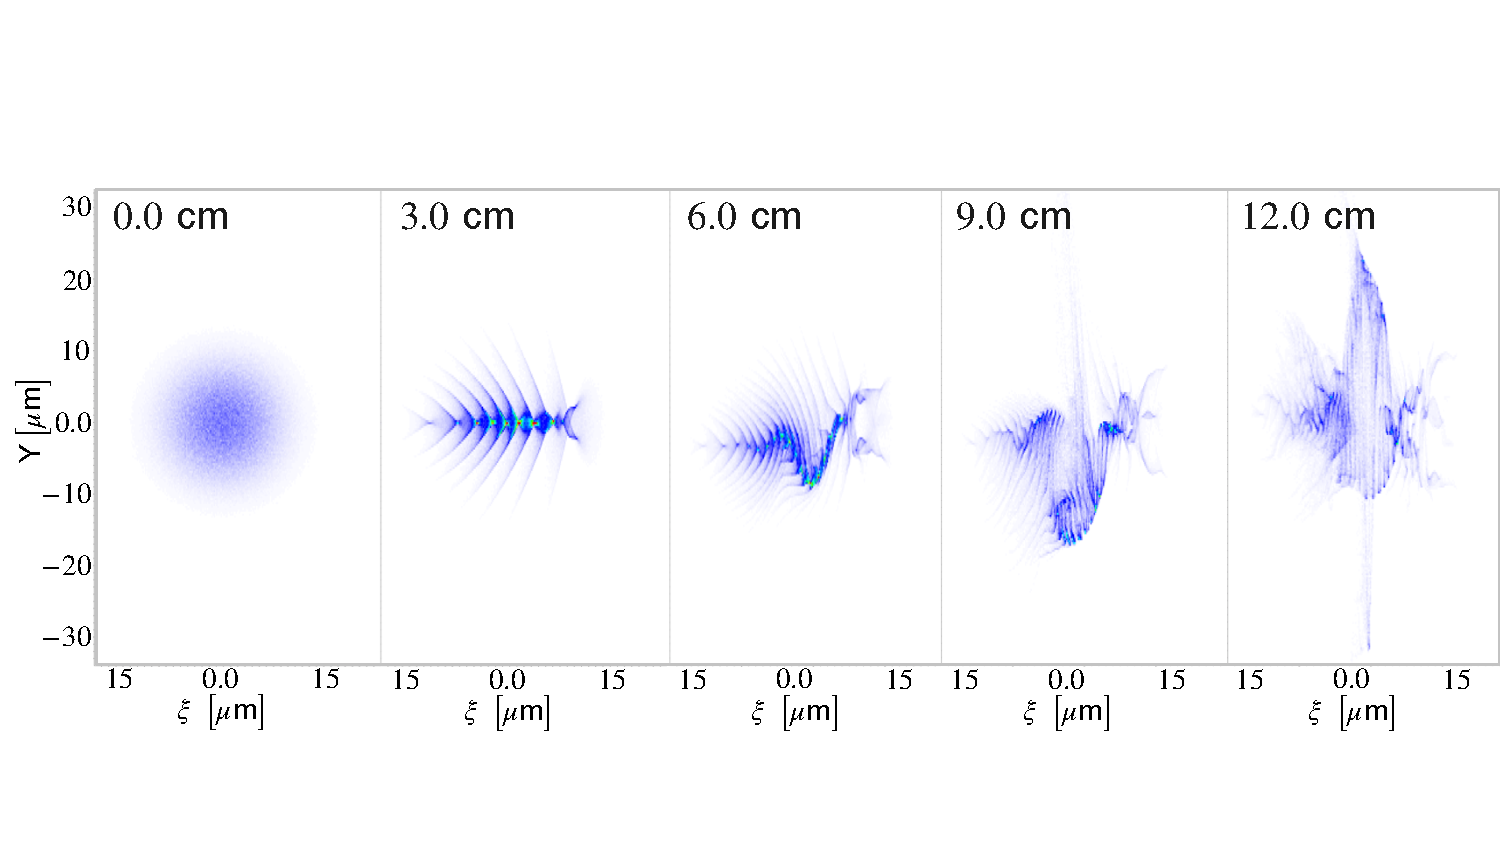
\includegraphics[width=\textwidth]{CherenkovInstability}
\caption{abc}
\end{figure}
%\section{Hybrid Scheme - Feasibility study}
%\subsection{Initialising a decelerated bunch}
%-Compare to actual already propagated bunch we want to simulate. See how quickly the uniform plasma resembles that of the plasma of the propagated simulation. If it takes long time then the laser results might not represent the real situation.  Compare simulations side by side as both real and initialised bunches propagate further, see if any deviations occur or if the bunch I set up is actually a fair approximation (compare energy, particle number etc.)
%\subsection{Introduction of co-propagating laser}
%- Results with respect to laser intensity/amplitude/wavelength as well as distance from bunch.


%\clearpage
%\hspace{-12pt}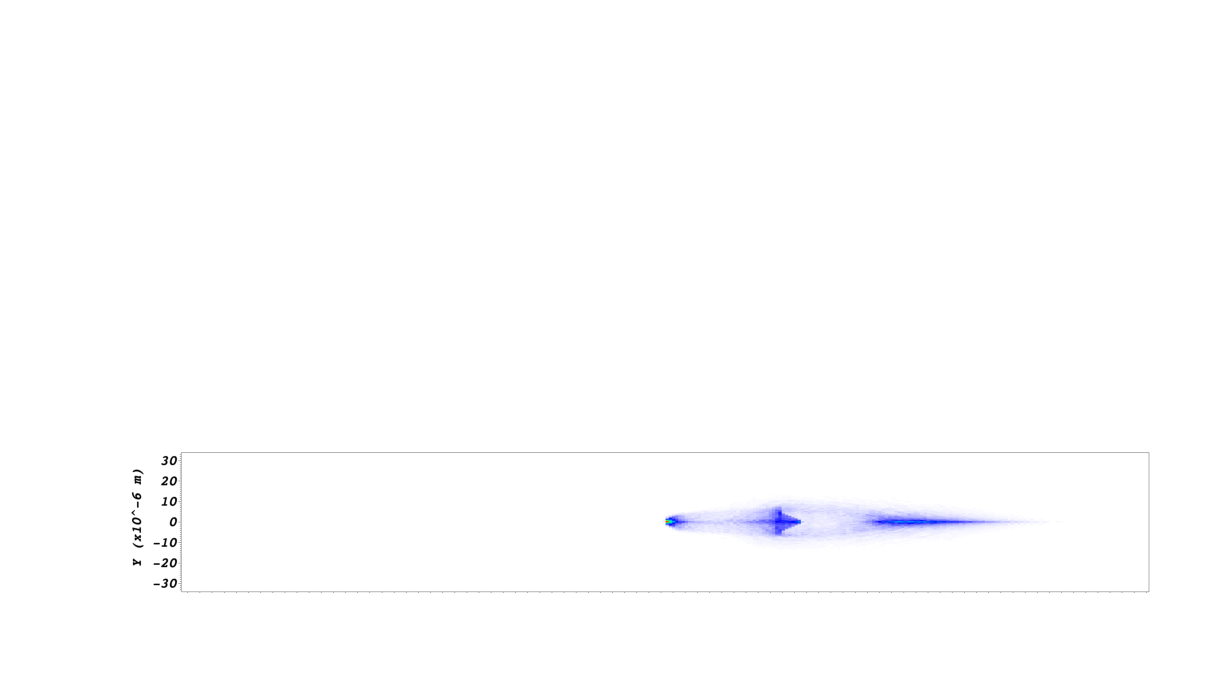
\includegraphics[width=\textwidth]{plot2linear}\vspace{-1pt}\\
%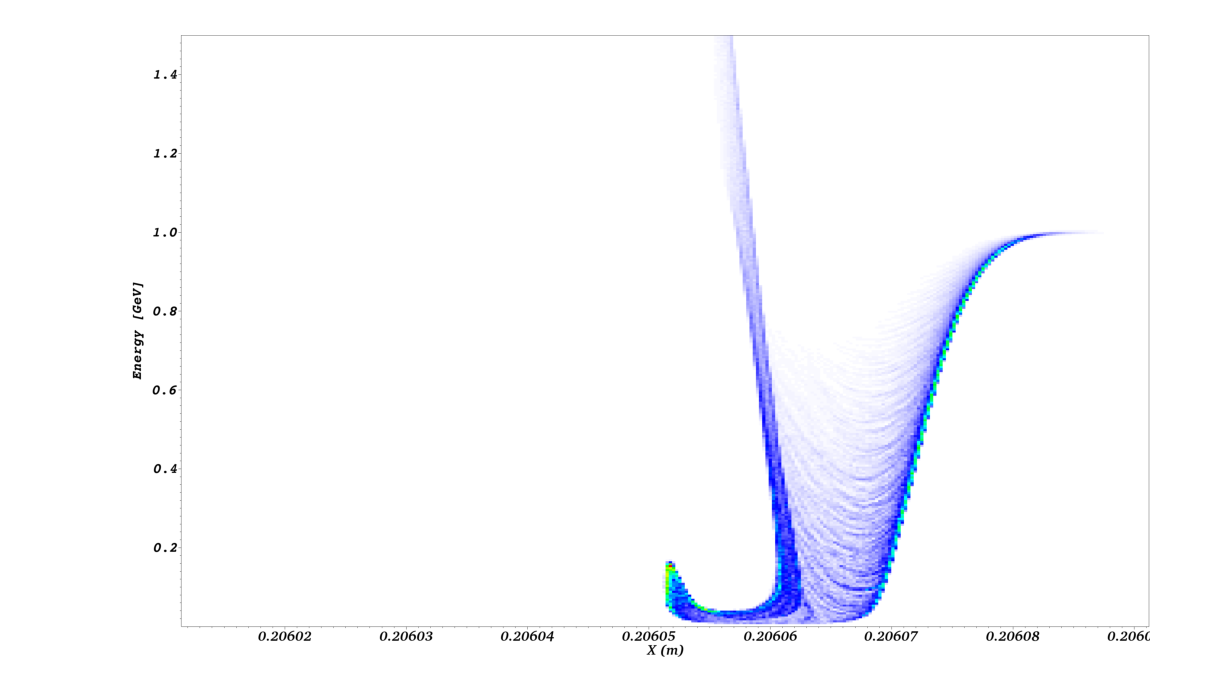
\includegraphics[width=\textwidth]{plot1linear}
%\clearpage
%\hspace{-12pt}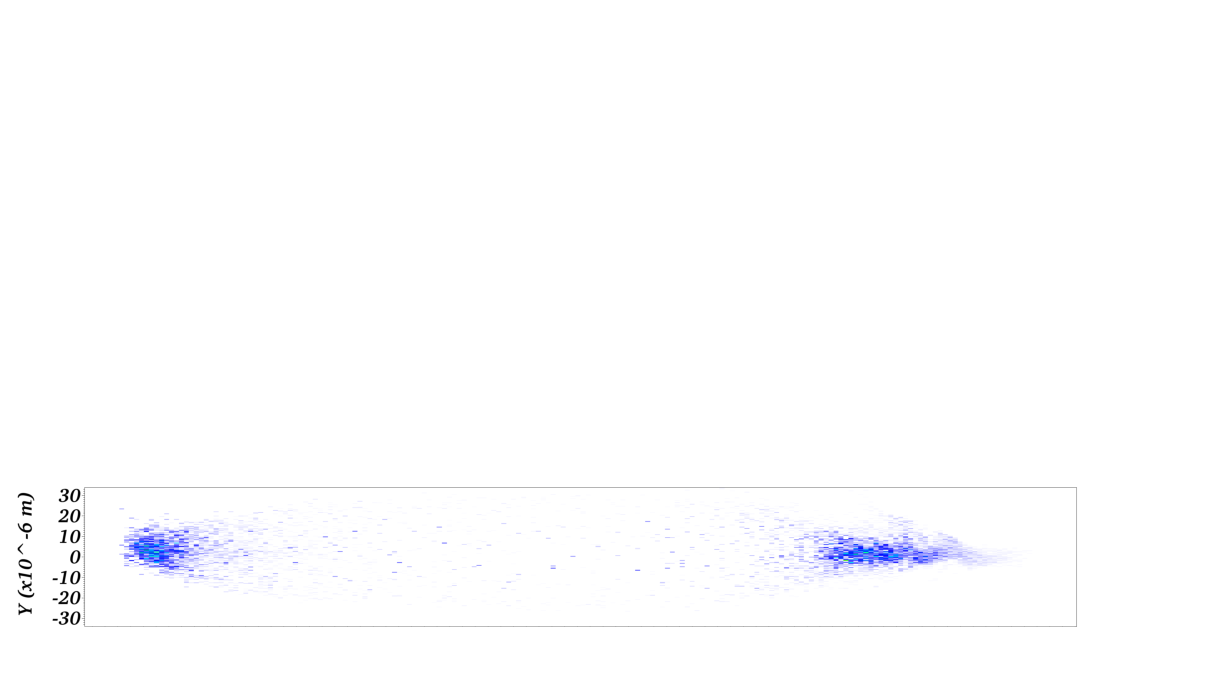
\includegraphics[width=\textwidth]{visit0022}\vspace{-1pt}\\
%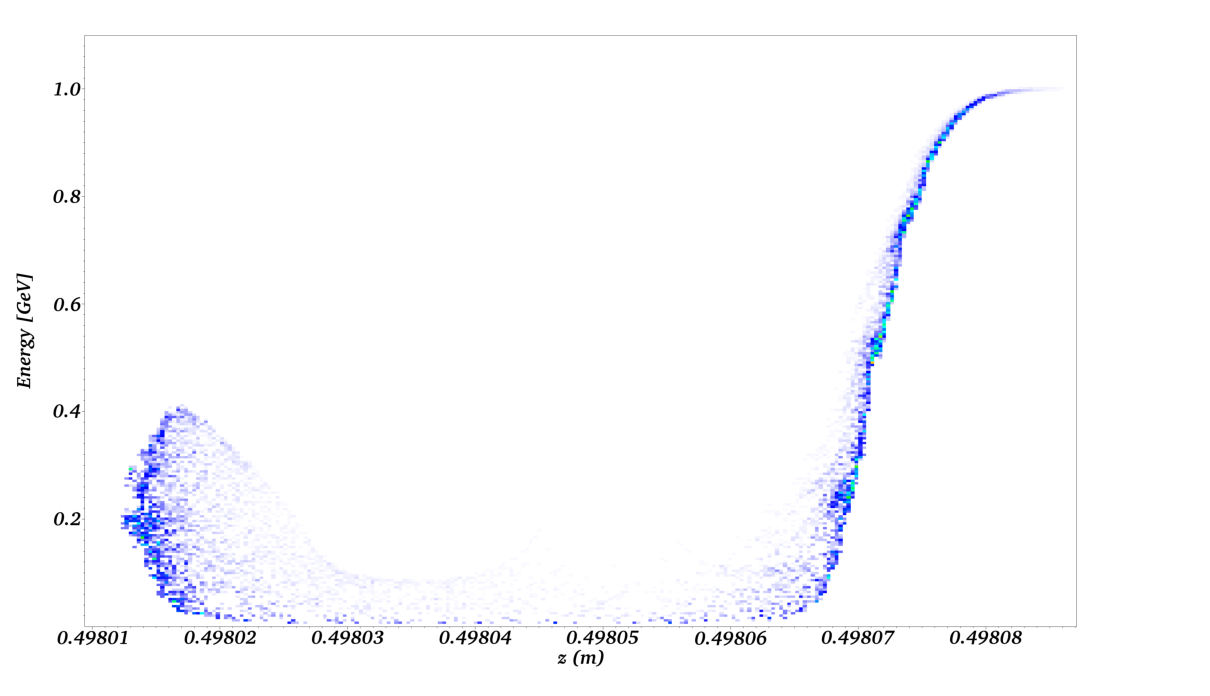
\includegraphics[width=\textwidth]{visit0020}